\subsection{Présentation}

	La cognition d'un agent se caractérise par l'ensemble des cognitons constituant l'esprit de l'agent, des plans susceptibles d'être effectués par l'agent ainsi que des liens entre ces composantes. 

\subsubsection{Cognitons}
	
	Les cognitons constituent l'ensemble des influences, internes ou externes, subies par l'agent. Cela peut représenter un savoir faire (ex : savoir cultiver un champ, faire du feu), une 
	

\subsection{Création d'une cognition}

La création d'une cognition complète regroupe donc la création de ces trois éléments dépendants les uns des autres. Il est donc nécessaire, avant de commencer la création d'un élément composant cette cognition , de connaitre  les dépendances entre les éléments de cette cognition. L'accès a l'interface de création d'une cognition se fait au moyen de l'onglet 
\includegraphics{images/ongcogni.png}. 

\subsubsection{Création d'un cogniton}

La création d'un nouveau cogniton se fait en cliquant sur l'icône 
\includegraphics{images/newcogni.png}. Un nouveau cogniton est alors créé sous la forme d'une ellipse portant le nom "Nouveau cogniton". 

Un clic droit sur ce dernier permet d'ouvrir l'interface d'édition. Le premier lien permet d'éditer le nom du cogniton, son type ( Belief si il s'agit d'une croyance de l'agent, Meme si il s'agit d'une croyance populaire, Percept si il s'agit d'une perception de l'agent, Skill si il s'agit d'une compétence ou d'un savoir-faire, Trait si il s'agit d'une caractéristique psychologique de l'agent et Culturon si il s'agit d'un cogniton partagé par un groupe) , et ses pourcentages de chances d'apparition au lancement de la simulation.

Viens ensuite l'édition des liens d'influence, a savoir, définir quels plans vont être influencés par ce cogniton et dans quelle mesure vont ils l'être. Pour cela, sélectionnez le plan a influencer ainsi que le poids de cette influence sur le plan en question. Une fois toutes les influences définies cliquez sur le bouton "OK" pour les enregistrer dans la simulation.

\begin{figure}[!h]
\begin{center}
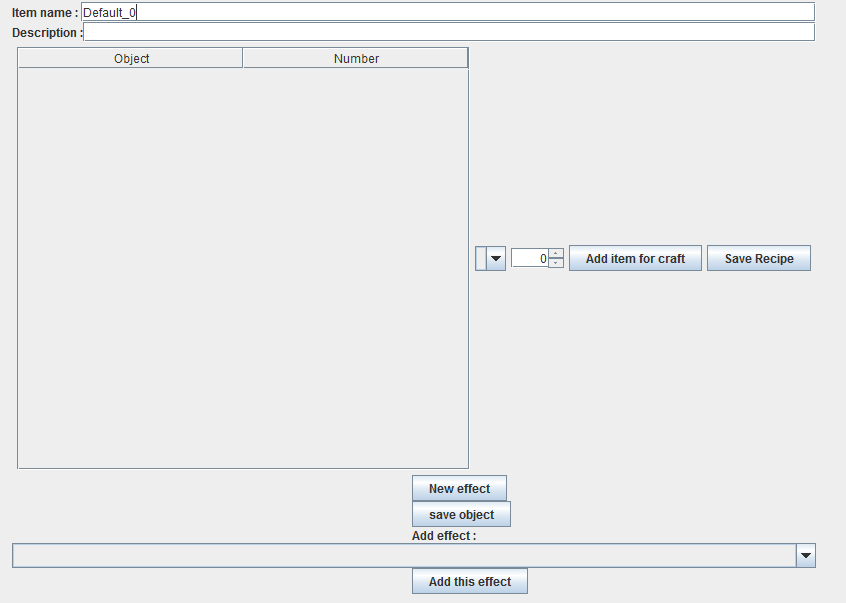
\includegraphics[scale = 0.7]{images/ecran.png}
\caption[eff]{Interface de création d'objet \\}
\label{Interface de création d'objet}
\end{center}
\end{figure}



\subsection{Observation durant la simulation}

Durant la simulation les objets portés par chaque agent peuvent être observés dans l'onglet "Agent". La colonne "Inventaire" contenant l'ensemble des objets portés par l'agent. Leurs différents effets peuvent être observés de façon indirecte en observant l'évolution des objets présents dans l'inventaire ainsi que les poids des cognitons et des plans présents dans l'esprit de l'agent et représentés dans ce même onglet.